%
% Documento: Introdução
%

\chapter{Sistemas Não Lineares}\label{chap:sistemas-nao-lineares}

O controle de sistemas não lineares tem sido alvo de extensiva pesquisa. Nos capítulos seguintes, este tema será abordado com maior profundido. Nesta seção, é mostrada  uma visão geral sobre sistemas não lineares e a relação deles com o projeto aqui proposto.

-- Adicionar Definição de um sistema não linear (com referência a livro)--

Este trabalho consiste na implementação de um controle para um quadrotor que é, também, um sistema não linear. Para contextualizar os sistemas não lineares, será abordado, além do quadrotor, o sistema de pêndulo invertido, que é um dos dos principais alvos de estudo dentre os sistemas desta categoria.

\section{Pêndulo Invertido}

-- Explicar o sistema de pêndulo invertido --

\subsection{Instabilidade do Sistema}

Ao utilizar o comando {\ttfamily open\textunderscore system('pendulum \textunderscore demo')}  no Matlab, abre-se uma janela com um diagrama de exemplo do próprio Matlab/Simulink para o controle de um pêndulo invertido. O diagrama exibido é mostrado na \autoref{fig:pendulum_matlab_full}.

\begin{figure}[!htb]
    \centering
    %\caption{Diagrama de blocos exibido no Matlab a partir do comando {\ttfamily open\textunderscore system('pendulum \textunderscore demo')} }
    \caption{Diagrama de blocos exibido no Matlab no exemplo de controle de pêndulo invertido}
    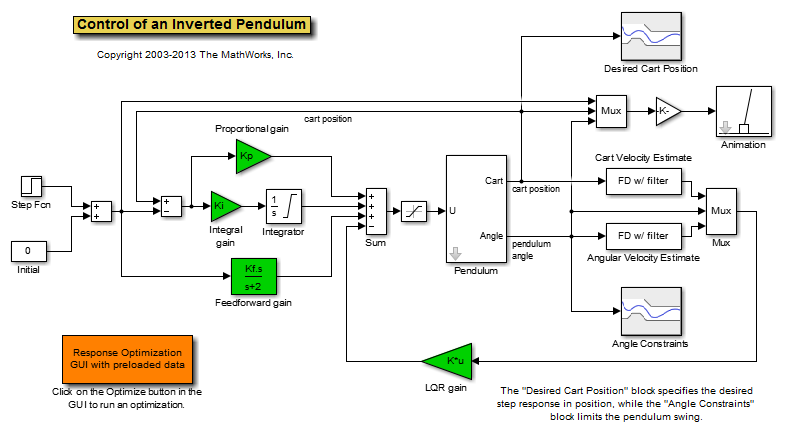
\includegraphics[width=1\textwidth]{./04-figuras/pendulum_matlab_full}
    \fonte{Nossa}
    \label{fig:pendulum_matlab_full}
\end{figure}

A partir deste exemplo, podemos extrair o bloco que implementa apenas a modelagem do sistema de pêndulo invertido, mostrado na \autoref{fig:pendulum_matlab_block}. A saída \textit{Cart} representa a posição do carro e a saída \textit{Angle} representa o ângulo de inclinação do pêndulo, em relação ao eixo y. A  \autoref{fig:pendulum_matlab_block_subsystem} mostra a modelagem interna ao blco que implementa o pêndulo invertido.

\begin{figure}[!htb]
    \centering
    \caption{Visão de caixa preta do modelo de pêndulo invertido}
    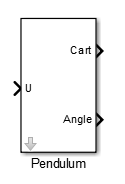
\includegraphics[width=0.2\textwidth]{./04-figuras/pendulum_matlab_block}
    \fonte{Nossa}
    \label{fig:pendulum_matlab_block}
\end{figure}

\begin{figure}[!htb]
    \centering
    \caption{Sistema implementado pela caixa preta do modelo de pêndulo invertido}
    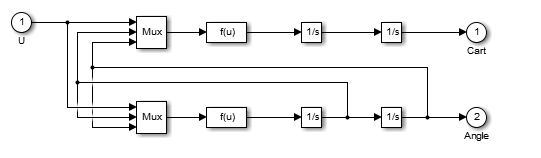
\includegraphics[width=0.9\textwidth]{./04-figuras/pendulum_matlab_block_subsystem}
    \fonte{Nossa}
    \label{fig:pendulum_matlab_block_subsystem}
\end{figure}

Utilizando o bloco mostrado na \autoref{fig:pendulum_matlab_block}, foi crido um sistema para mostrar a instabilidade intrínseca ao sistema de pêndulo invertido. Para tanto, aplicou-se uma entrada degrau ao sistema. O diagrama em blocos do sistema é mostrado na \autoref{fig:pendulum_matlab_step_diagram}.

\begin{figure}[!htb]
    \centering
    \caption{Sistema implementado para mostrar instabilidade do pêndulo invertido}
    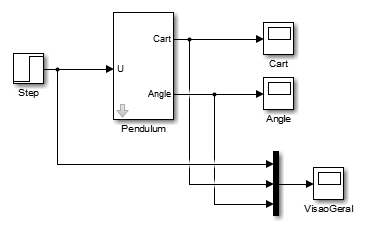
\includegraphics[width=0.7\textwidth]{./04-figuras/pendulum_matlab_step_diagram}
    \fonte{Nossa}
    \label{fig:pendulum_matlab_step_diagram}
\end{figure}

Diferentes simulações foram feitas. A \autoref{fig:pendulum_matlab_step_diagram_geral_step1} mostra o resultado para entrada degrau com amplitude 1 e tempo de amostragem de 10 ms. A \autoref{fig:pendulum_matlab_step_diagram_geral_step0_1} mostra o resultado para entrada degrau com amplitude 0.1 e tempo de amostragem de 10 ms. A \autoref{fig:pendulum_matlab_step_diagram_geral_step1_5s} e a  \autoref{fig:pendulum_matlab_step_diagram_geral_step0_1_5s} mostram os resultados para entrada degrau com valores 1 e 0.1, respectivamente, com tempo de amostragem de 5 ms. A \autoref{fig:pendulum_matlab_subtitles} mostra a legenda para todos estes resultados.


\begin{figure}[!htb]
    \centering
    \caption{Legenda para as simulações de pêndulo invertido no Matlab}
    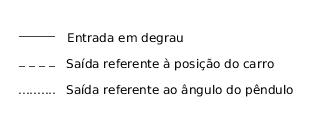
\includegraphics[width=0.6\textwidth]{./04-figuras/pendulum_matlab_subtitles}
    \fonte{Nossa}
    \label{fig:pendulum_matlab_subtitles}
\end{figure}

\begin{figure}[!htb]
    \centering
    \caption{Resposta do pêndulo a um degrau com amplitude 1 com tempo de amostragem de 10 ms}
    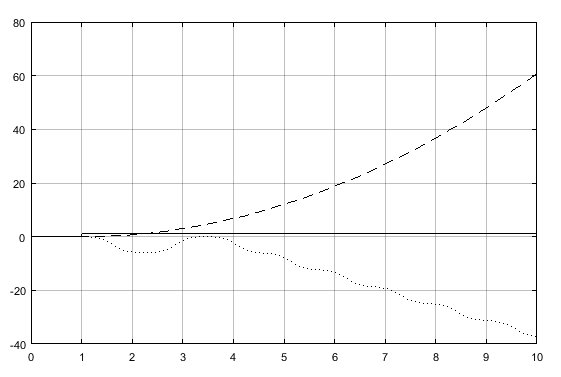
\includegraphics[width=0.7\textwidth]{./04-figuras/pendulum_matlab_step_diagram_geral_step1}
    \fonte{Nossa}
    \label{fig:pendulum_matlab_step_diagram_geral_step1}
\end{figure}

\begin{figure}[!htb]
    \centering
    \caption{Resposta do pêndulo a um degrau com amplitude 0,1 com tempo de amostragem de 10 ms}
    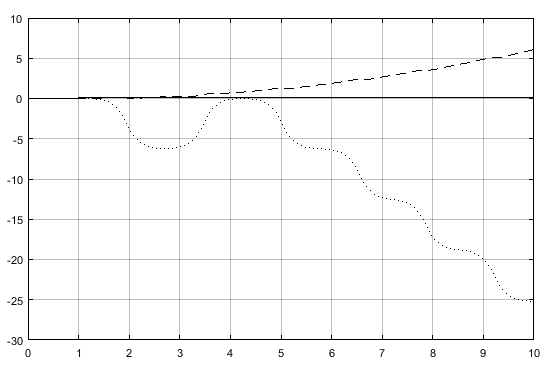
\includegraphics[width=0.7\textwidth]{./04-figuras/pendulum_matlab_step_diagram_geral_step0_1}
    \fonte{Nossa}
    \label{fig:pendulum_matlab_step_diagram_geral_step0_1}
\end{figure}

\begin{figure}[!htb]
    \centering
    \caption{Resposta do pêndulo a um degrau com amplitude 1 com tempo de amostragem de 5 ms}
    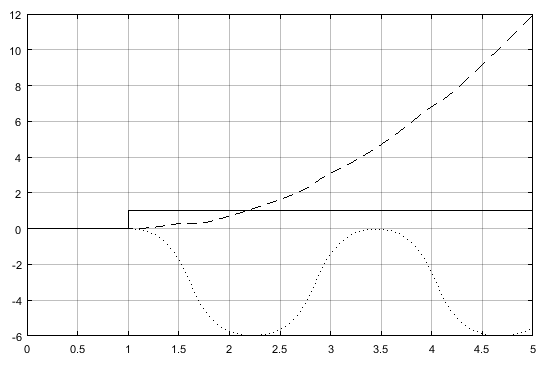
\includegraphics[width=0.7\textwidth]{./04-figuras/pendulum_matlab_step_diagram_geral_step1_5s}
    \fonte{Nossa}
    \label{fig:pendulum_matlab_step_diagram_geral_step1_5s}
\end{figure}

\begin{figure}[!htb]
    \centering
    \caption{Resposta do pêndulo a um degrau com amplitude 0,1 com tempo de amostragem de 5 ms}
    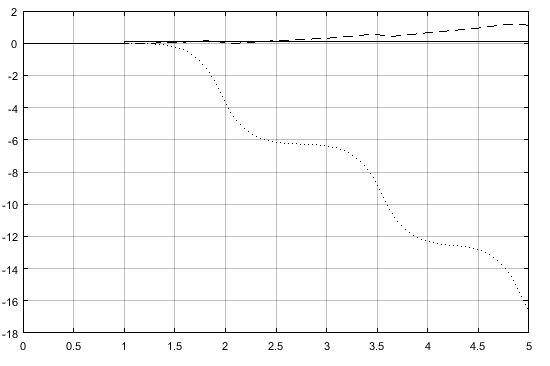
\includegraphics[width=0.7\textwidth]{./04-figuras/pendulum_matlab_step_diagram_geral_step0_1_5s}
    \fonte{Nossa}
    \label{fig:pendulum_matlab_step_diagram_geral_step0_1_5s}
\end{figure}

%pendulum_matlab_step_diagram_geral_step1
%pendulum_matlab_step_diagram_geral_step0_1
%pendulum_matlab_step_diagram_geral_step1_5s
%pendulum_matlab_step_diagram_geral_step0_1_5s

Como se pode ver, em todos os casos é verificada a instabilidade do sistema. A partir de um estímulo, neste caso causado pela entrada em degrau, o sistema diverge tanto com relação à posição do carro, quanto ao ângulo do pêndulo.

%\section{Helicóptero Quadrotor}

%-- Explicar o sistema de um quadricóptero --

%Seção ainda não escrita.

%\subsection{Instabilidade do Sistema}

%Seção ainda não escrita.
